% (find-LATEX "2021-1-C3-visualizar-limites.tex")
% (defun c () (interactive) (find-LATEXsh "lualatex -record 2021-1-C3-visualizar-limites.tex" :end))
% (defun C () (interactive) (find-LATEXsh "lualatex 2021-1-C3-visualizar-limites.tex" "Success!!!"))
% (defun D () (interactive) (find-pdf-page      "~/LATEX/2021-1-C3-visualizar-limites.pdf"))
% (defun d () (interactive) (find-pdftools-page "~/LATEX/2021-1-C3-visualizar-limites.pdf"))
% (defun e () (interactive) (find-LATEX "2021-1-C3-visualizar-limites.tex"))
% (defun o () (interactive) (find-LATEX "2021-1-C3-visualizar-limites.tex"))
% (defun u () (interactive) (find-latex-upload-links "2021-1-C3-visualizar-limites"))
% (defun v () (interactive) (find-2a '(e) '(d)))
% (defun d0 () (interactive) (find-ebuffer "2021-1-C3-visualizar-limites.pdf"))
% (defun cv () (interactive) (C) (ee-kill-this-buffer) (v) (g))
%          (code-eec-LATEX "2021-1-C3-visualizar-limites")
% (find-pdf-page   "~/LATEX/2021-1-C3-visualizar-limites.pdf")
% (find-sh0 "cp -v  ~/LATEX/2021-1-C3-visualizar-limites.pdf /tmp/")
% (find-sh0 "cp -v  ~/LATEX/2021-1-C3-visualizar-limites.pdf /tmp/pen/")
%     (find-xournalpp "/tmp/2021-1-C3-visualizar-limites.pdf")
%   file:///home/edrx/LATEX/2021-1-C3-visualizar-limites.pdf
%               file:///tmp/2021-1-C3-visualizar-limites.pdf
%           file:///tmp/pen/2021-1-C3-visualizar-limites.pdf
% http://angg.twu.net/LATEX/2021-1-C3-visualizar-limites.pdf
% (find-LATEX "2019.mk")
% (find-CN-aula-links "2021-1-C3-visualizar-limites" "3" "c3m211vl" "c3vl")
%
% Video (nao fiz):
% (find-ssr-links "c3m211vl" "2021-1-C3-visualizar-limites")
% (code-video     "c3m211vlvideo" "$S/http/angg.twu.net/eev-videos/2021-1-C3-visualizar-limites.mp4")
% (find-c3m211vlvideo "0:00")

% «.defs»		(to "defs")
% «.title»		(to "title")
% «.na-aula-passada»	(to "na-aula-passada")
% «.tipos»		(to "tipos")
% «.intro-exercs»	(to "intro-exercs")
% «.exercicio-1»	(to "exercicio-1")
% «.exercicio-2»	(to "exercicio-2")
% «.exercicio-3»	(to "exercicio-3")
% «.exercicio-4»	(to "exercicio-4")
% «.exercicio-5»	(to "exercicio-5")
%
% «.djvuize»		(to "djvuize")

\documentclass[oneside,12pt]{article}
\usepackage[colorlinks,citecolor=DarkRed,urlcolor=DarkRed]{hyperref} % (find-es "tex" "hyperref")
\usepackage{amsmath}
\usepackage{amsfonts}
\usepackage{amssymb}
\usepackage{pict2e}
\usepackage[x11names,svgnames]{xcolor} % (find-es "tex" "xcolor")
\usepackage{colorweb}                  % (find-es "tex" "colorweb")
%\usepackage{tikz}
%
% (find-dn6 "preamble6.lua" "preamble0")
%\usepackage{proof}   % For derivation trees ("%:" lines)
%\input diagxy        % For 2D diagrams ("%D" lines)
%\xyoption{curve}     % For the ".curve=" feature in 2D diagrams
%
\usepackage{edrx15}               % (find-LATEX "edrx15.sty")
\input edrxaccents.tex            % (find-LATEX "edrxaccents.tex")
\input edrxchars.tex              % (find-LATEX "edrxchars.tex")
\input edrxheadfoot.tex           % (find-LATEX "edrxheadfoot.tex")
\input edrxgac2.tex               % (find-LATEX "edrxgac2.tex")
%
%\usepackage[backend=biber,
%   style=alphabetic]{biblatex}            % (find-es "tex" "biber")
%\addbibresource{catsem-slides.bib}        % (find-LATEX "catsem-slides.bib")
%
% (find-es "tex" "geometry")
\usepackage[a6paper, landscape,
            top=1.5cm, bottom=.25cm, left=1cm, right=1cm, includefoot
           ]{geometry}
%
\begin{document}

%\catcode`\^^J=10
%\directlua{dofile "dednat6load.lua"}  % (find-LATEX "dednat6load.lua")

% %L dofile "edrxtikz.lua"  -- (find-LATEX "edrxtikz.lua")
% %L dofile "edrxpict.lua"  -- (find-LATEX "edrxpict.lua")
% \pu

% «defs»  (to ".defs")
% (find-LATEX "edrx15.sty" "colors-2019")
\long\def\ColorRed   #1{{\color{Red1}#1}}
\long\def\ColorViolet#1{{\color{MagentaVioletLight}#1}}
\long\def\ColorViolet#1{{\color{Violet!50!black}#1}}
\long\def\ColorGreen #1{{\color{SpringDarkHard}#1}}
\long\def\ColorGreen #1{{\color{SpringGreenDark}#1}}
\long\def\ColorGreen #1{{\color{SpringGreen4}#1}}
\long\def\ColorGray  #1{{\color{GrayLight}#1}}
\long\def\ColorGray  #1{{\color{black!30!white}#1}}
\long\def\ColorBrown #1{{\color{Brown}#1}}
\long\def\ColorBrown #1{{\color{brown}#1}}
\long\def\ColorOrange#1{{\color{orange}#1}}

\long\def\ColorShort #1{{\color{SpringGreen4}#1}}
\long\def\ColorLong  #1{{\color{Red1}#1}}

\def\frown{\ensuremath{{=}{(}}}
\def\True {\mathbf{V}}
\def\False{\mathbf{F}}
\def\D    {\displaystyle}

\def\rq{\ColorRed{?}}
\def\undq#1{\underbrace{#1}_{\rq}}


\def\drafturl{http://angg.twu.net/LATEX/2021-1-C3.pdf}
\def\drafturl{http://angg.twu.net/2021.1-C3.html}
\def\draftfooter{\tiny \href{\drafturl}{\jobname{}} \ColorBrown{\shorttoday{} \hours}}



%  _____ _ _   _                               
% |_   _(_) |_| | ___   _ __   __ _  __ _  ___ 
%   | | | | __| |/ _ \ | '_ \ / _` |/ _` |/ _ \
%   | | | | |_| |  __/ | |_) | (_| | (_| |  __/
%   |_| |_|\__|_|\___| | .__/ \__,_|\__, |\___|
%                      |_|          |___/      
%
% «title»  (to ".title")
% (c3m211vlp 1 "title")
% (c3m211vla   "title")

\thispagestyle{empty}

\begin{center}

\vspace*{1.2cm}

{\bf \Large Cálculo 3 - 2021.1}

\bsk

Aula 3: como visualizar limites

\bsk

Eduardo Ochs - RCN/PURO/UFF

\url{http://angg.twu.net/2021.1-C3.html}

\end{center}

\newpage

% (find-books "__analysis/__analysis.el" "bortolossi")
% (find-bortolossi6page (+ -186 187) "6. Curvas parametrizadas, transformações lineares...")
% (find-bortolossi6page (+ -186 188)   "traço")
% (find-bortolossi6page (+ -186 195)   "Figura 6.6. Traço da hélice")
% (find-bortolossi6page (+ -186 197) "6.2 O vetor tangente a uma curva parametrizada")
% (find-bortolossi6page (+ -186 199)   "limite de vetores secantes")
% (find-bortolossi6page (+ -186 215)   "A ciclóide")
% (find-bortolossi6page (+ -186 217)   "O vetor aceleração")

% (find-bortolossi6page (+ -186 199) "limite de vetores secantes")

% «na-aula-passada»  (to ".na-aula-passada")
% (c3m211vlp 2 "na-aula-passada")
% (c3m211vla   "na-aula-passada")

Na aula passada eu disse que o {\sl vetor velocidade} da trajetória
%
$$P(t) = (\cos t, \sen t)$$

era o {\sl vetor}
%
$$\begin{array}{rcl}
  P'(t) &=& (\cos' t, \sen' t) \\
        &=& (-\sen t, \cos t) \\
  \end{array}
$$

que na verdade deve ser escrito como:
%
$$\begin{array}{rcl}
  \Vec{P'}(t) &=& \VEC{-\sen t, \cos t} \\
  \end{array}
$$

mas eu esqueci as setinhas --- e eu fiquei devendo a explicação

de porque é que cada $P'(t)$ deve ser um vetor e não um ponto.

Hoje a gente vai ver como o Bortolossi define esse $\Vec{P'}(t)$

como um limite, e vamos ver algumas técnicas pra decifrar

a linguagem, a notação e as figuras do livro dele.

\newpage

% «tipos»  (to ".tipos")
% (c3m211vlp 3 "tipos")
% (c3m211vla   "tipos")
% (find-LATEXgrep "grep --color=auto -nH --null -e tipos 2020-2-C3*.tex")
% (c3m202rcadeia1p 8 "tipos")
% (c3m202rcadeia1a   "tipos")

{\bf Tipos}

\ssk

{\bf TUDO} que nós vamos fazer em Cálculo 3 pode ser {\sl visualizado}
e {\sl tipado}. Você já viu um pouco de tipos em {\tt C} e em Física;
em Física os ``tipos'' são parcialmente determinados pelas unidades
--- metros são distância, segundos são tempo, metros/segundo é uma
unidade de velocidade, e assim por diante...

% (find-bortolossi5page (+ -162 164) "5.2. Definições e exemplos")
% (find-bortolossi5page (+ -162 165)   "Fig. 5.2: Interpretação geométrica")

Dê uma olhada nas páginas 164 a 166 do capítulo 5 do Bortolossi. Todas
as expressões que aparecem lá podem ser ``tipadas'' e interpretadas
como posições no eixo $x$ (ou no eixo $y$, ou no eixo $y$), ou como
distâncias no eixo $x$ (ou no eixo $y$, ou $z$), ou como {\sl
  inclinações}... vamos ver os detalhes disto aos poucos.

\newpage

% «intro-exercs»  (to ".intro-exercs")
% (c3m211vlp 4 "intro-exercs")
% (c3m211vla   "intro-exercs")

Nos próximos exercícios você vai tentar ``tipar'' cada subexpressão
deles. Escreva os seus tipos nos lugares em que eu pus as `$\rq$'s.
Use português, improvise o quanto precisar, e compare o seu modo de
escrever os tipos com os dos seus colegas. Lembre que aqui nós estamos
tentando fazer explicitamente, num diagrama, algo que os livros fazem
em poucas frases de texto fingindo que é algo óbvio.

Se você tiver dificuldade de fazer o caso geral faça um caso
particular primeiro.

\newpage

% «exercicio-1»  (to ".exercicio-1")
% (c3m211vlp 5 "exercicio-1")
% (c3m211vla   "exercicio-1")
% (c3m202rcadeia1p 32 "tipos-de-novo")
% (c3m202rcadeia1a    "tipos-de-novo")


{\bf Exercício 1}

Digamos que $f(x)=x^2$ e que $y=f(x)$. 

Se você tiver dificuldade de pensar no caso geral

faça $x_0=1$ e $Δx=0.1$.

$$\undq{
  \undq{(\undq{\undq{f}(\undq{\undq{x_0} + \undq{Δx}})}
        - \undq{\undq{f}(\undq{x_0})})} / \undq{Δx}
  }
$$


\newpage

% «exercicio-2»  (to ".exercicio-2")
% (c3m211vlp 6 "exercicio-2")
% (c3m211vla   "exercicio-2")

{\bf Exercício 2}

Digamos que $f(t)=\cos t$, $g(t)=\sen t$, e $P(t)=(f(t),g(t))$. 

Se você tiver dificuldade de pensar no caso geral

faça $t_0=\fracπ2$ e $Δt=0.1$.

$$\undq{
  \undq{(\undq{\undq{P}(\undq{\undq{t_0} + \undq{Δt}})}
        - \undq{\undq{P}(\undq{t_0})})} / \undq{Δt}
  }
$$

\newpage

% «exercicio-3»  (to ".exercicio-3")
% (c3m211vlp 7 "exercicio-3")
% (c3m211vla   "exercicio-3")

{\bf Exercício 3}

Digamos que $f(t)=\cos t$, $g(t)=\sen t$, e $P(t)=(f(t),g(t))$. 

Se você tiver dificuldade de pensar no caso geral

faça $t_0=\fracπ2$ e $Δt=0.1$.
%
$$\undq{\undq{P}(\undq{\undq{t_0} + \undq{Δt}})}
  =
  \undq{
    ( \undq{\undq{f}(\undq{\undq{t_0} + \undq{Δt}})},
      \undq{\undq{g}(\undq{\undq{t_0} + \undq{Δt}})} )
  }
$$

\newpage

% «exercicio-4»  (to ".exercicio-4")
% (c3m211vlp 8 "exercicio-4")
% (c3m211vla   "exercicio-4")
% (find-bortolossi6page (+ -186 197) "6.2 O vetor tangente a uma curva parametrizada")
% (find-bortolossi6page (+ -186 198)   "mas este vetor limite pode ser calculado")
% (find-bortolossi6page (+ -186 199)   "limite de vetores secantes")

Agora nós vamos começar a ver como decifrar definições

como a das páginas 197--198 do capítulo 6 do Bortolossi.

Ele faz tudo de um jeito bem geral, e ele usa $\R^m$ ao invés

de $\R^2$ ou $\R^3$.

\bsk

{\bf Exercício 4}

Reescreva a conta grande no meio da página 198 do Bortolossi

substituindo $t_0$ por $\fracπ2$, $h_j$ por $ε$,
$x_1(t)$ por $\cos t$, $x_2(t)$ por $\sen t$,

e $m$ por 2. Obs: os `$\ldots$' vão sumir.

\newpage

O livro do Bortolossi tem essa figura daqui na página 199:
%
% (find-latexscan-links "C3" "20210625_bortolossi_p199")
% (find-xpdf-page "~/LATEX/2021-1-C3/20210625_bortolossi_p199.pdf")
$$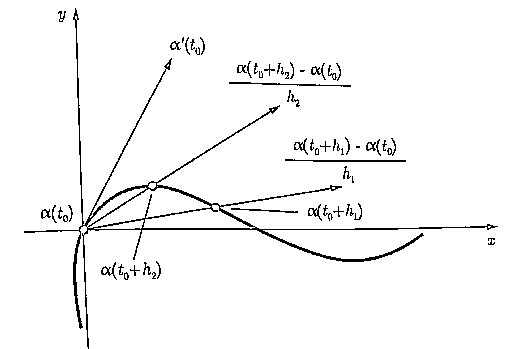
\includegraphics[height=4.5cm]{2021-1-C3/20210625_bortolossi_p199.pdf}$$

Isso é um desenho de vetor velocidade como limite de retas secantes
num caso geral -- o Bortolossi não nos diz quem são $α:\R→\R^2$, nem
$t_0$, nem a sequência $(h_1, h_2, h_3, \ldots)$, e isso sugere que
essa figura vai valer pra quaisquer $α$, $t_0$ e $(h_1, h_2, \ldots)$,
com as devidas adaptações...

\newpage

% «exercicio-5»  (to ".exercicio-5")
% (c3m211vlp 10 "exercicio-5")
% (c3m211vla    "exercicio-5")

{\bf Exercício 5}

Aqui nós vamos tentar fazer uma figura parecida com

a do caso anterior, mas com $α(t) = (\cos t, \sen t)$, $t_0=\fracπ2$,

$h_0 = \fracπ2$, $0 < \ldots < h_3 < h_2 < h_1 < h_0$, $\lim_{j→∞} h_j = 0$.

Comece com esta figura aqui,
%
% (find-latexscan-links "C3" "20210625_bortolossi_p199_hack")
% (find-xpdf-page "~/LATEX/2021-1-C3/20210625_bortolossi_p199_hack.pdf")
$$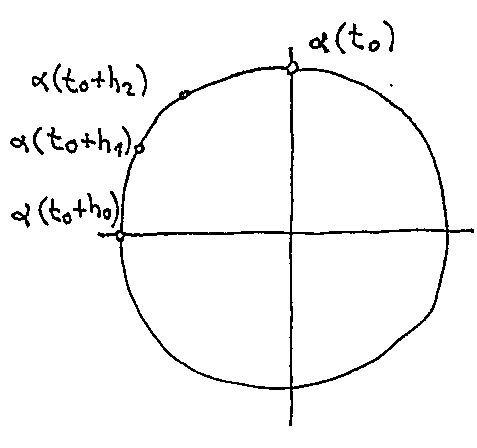
\includegraphics[height=3cm]{2021-1-C3/20210625_bortolossi_p199_hack.pdf}$$

e encontre valores razoáveis para $h_1$, $h_2$ e $h_3$ que te

permitam completar o desenho no olhômetro fazendo

as contas de cabeça com aproximações bem grosseiras.



\newpage


(Não olhe pro que vem depois daqui)



\newpage


$$\undq{
  \undq{(\undq{F(\undq{\undq{\undq{x_0} + \undq{Δx}},\undq{y_0}})}
        - \undq{F(\undq{\undq{x_0},\undq{y_0}})})} / \undq{Δx}
  }
$$


%\printbibliography

\GenericWarning{Success:}{Success!!!}  % Used by `M-x cv'

\end{document}


%  ____  _             _         
% |  _ \(_)_   ___   _(_)_______ 
% | | | | \ \ / / | | | |_  / _ \
% | |_| | |\ V /| |_| | |/ /  __/
% |____// | \_/  \__,_|_/___\___|
%     |__/                       
%
% «djvuize»  (to ".djvuize")
% (find-LATEXgrep "grep --color -nH --null -e djvuize 2020-1*.tex")

 (eepitch-shell)
 (eepitch-kill)
 (eepitch-shell)
# (find-fline "~/2021.1-C3/")
# (find-fline "~/LATEX/2021-1-C3/")
# (find-fline "~/bin/djvuize")

cd /tmp/
for i in *.jpg; do echo f $(basename $i .jpg); done

f () { rm -fv $1.png $1.pdf; djvuize $1.pdf }
f () { rm -fv $1.png $1.pdf; djvuize WHITEBOARDOPTS="-m 1.0" $1.pdf; xpdf $1.pdf }
f () { rm -fv $1.png $1.pdf; djvuize WHITEBOARDOPTS="-m 0.5" $1.pdf; xpdf $1.pdf }
f () { rm -fv $1.png $1.pdf; djvuize WHITEBOARDOPTS="-m 0.25" $1.pdf; xpdf $1.pdf }
f () { cp -fv $1.png $1.pdf       ~/2021.1-C3/
       cp -fv        $1.pdf ~/LATEX/2021-1-C3/
       cat <<%%%
% (find-latexscan-links "C3" "$1")
%%%
}

f 20210625_bortolossi_p199
f 20210625_bortolossi_p199_hack

f 20201213_area_em_funcao_de_theta
f 20201213_area_em_funcao_de_x
f 20201213_area_fatias_pizza



%  __  __       _        
% |  \/  | __ _| | _____ 
% | |\/| |/ _` | |/ / _ \
% | |  | | (_| |   <  __/
% |_|  |_|\__,_|_|\_\___|
%                        
% <make>

 (eepitch-shell)
 (eepitch-kill)
 (eepitch-shell)
# (find-LATEXfile "2019planar-has-1.mk")
make -f 2019.mk STEM=2021-1-C3-visualizar-limites veryclean
make -f 2019.mk STEM=2021-1-C3-visualizar-limites pdf

% Local Variables:
% coding: utf-8-unix
% ee-tla: "c3vl"
% ee-tla: "c3m211vl"
% End:
